\documentclass[a4paper,11pt]{report}
\usepackage[utf8]{inputenc}
\usepackage[T1]{fontenc}
\usepackage{graphicx}
\usepackage[defaultsans]{opensans}
\usepackage{enumitem}
\usepackage{listings}
\usepackage[utf8]{inputenc}
\usepackage[francais, english]{babel}
\usepackage{parskip}
\setlength{\parskip}{10pt plus 0pt minus 0pt}
\usepackage[left=2cm,right=3cm]{geometry}

\usepackage{color}
\definecolor{editorLightGray}{cmyk}{0.05, 0.05, 0.05, 0.1}
\definecolor{editorGray}{cmyk}{0.6, 0.55, 0.55, 0.2}
\definecolor{editorPurple}{cmyk}{0.5, 1, 0, 0}
\definecolor{editorWhite}{cmyk}{0, 0, 0, 0}
\definecolor{editorBlack}{cmyk}{1, 1, 1, 1}
\definecolor{editorOrange}{cmyk}{0, 0.8, 1, 0}
\definecolor{editorBlue}{cmyk}{1, 0.6, 0, 0}
\definecolor{editorPink}{cmyk}{0, 0.6745, 0.5608, 0}

 \lstset{
  language=html,
  tagstyle=\color{editorBlue},
  basicstyle={\small\ttfamily},
  identifierstyle=\color{editorOrange},
  keywordstyle=\color{editorPink},
  commentstyle=\color{editorGray},
  stringstyle=\color{editorPurple}
}

\usepackage{upquote}
\usepackage{listings}

\DeclareRobustCommand\ebseries{\fontseries{eb}\selectfont}
\DeclareRobustCommand\sbseries{\fontseries{sb}\selectfont}
\DeclareRobustCommand\ltseries{\fontseries{l}\selectfont}
\DeclareRobustCommand\clseries{\fontseries{cl}\selectfont}

\DeclareTextFontCommand{\texteb}{\ebseries}
\DeclareTextFontCommand{\textsb}{\sbseries}
\DeclareTextFontCommand{\textlt}{\ltseries}
\DeclareTextFontCommand{\textcl}{\clseries}


\begin{document}


\chapter{Introduction}


\chapter{Le contexte du travail}
\section{Le cahier des charges ?}
\section{L'architecture de la plateforme cible}
\section{Le framework Angularjs ?}

AngularJS\footnote{url de angular} est un framework écrit en javascript par Google libre et
open-source qui permet d'améliorer, au même titre que JQUERY, la
syntaxe de javascript ainsi que la productivité du
développeur. Il étend le HTML pour le rendre dynamique, et permet de
développer ses propres balises et attributs HTML. C’est un framework
qui se veut extensible et qui pousse vers un développement structuré, 
en couches, le but n’étant pas d’ajouter de simples animations au DOM,
mais bien d’apporter un aspect applicatif au front-end.


\subsection{Concept}
Angular est construit autour de concepts et de bonnes pratiques
incontournables dans le monde du développement web.

\begin{itemize}
 \item Architecture {\tt Modèle-Vue-Contrôller} (MVC) :
  si vous connaissez le développement, vous avez sûrement entendu parler
  de ce type d'architecture incontournable qui consiste à avoir une stricte
  séparation entre les données (Modèle), la présentation des données (Vue),
  et les actions que l'on peut effectuer sur ces données (Contrôleur).
  \item Le {\tt data-binding bidirectionnel} est un moyen de lier la partie vue
  à la partie logique. En d'autres termes, grâce à cela, les éléments de 
  votre code HTML seront liés à votre contrôleur JavaScript est rendu 
  possible grâce au scope.  Le scope est le “liant” d’une application AngularJS,
  c’est lui qui contient les variables et fonctions qui font la liaison entre vues 
  et contrôleurs (ou autres). Il permet donc aux données de pouvoir être mises à 
  jour par les vues et par le modèle.
  \item {\tt L’injection de dépendances} permet de charger certaines parties de 
  l’application seulement quand c’est nécessaire.
  \item La manipulation du DOM au moyen de directives : AngularJS dispose d'un grand
  nombre de directives permettant de manipuler le DOM et offre aussi la possibilité 
  aux dévelopeurs d'écrire leurs propres directives.
  \item Le Routage, le module de routage de Angularjs est l'un des composants clés 
  lui permettant de créer des applications {\tt Single Page Application} (SPA). En effet,
  si le développeur veut pouvoir naviguer sur plusieurs pages et en même temps en faire une
  application monopage, il peut utiliser le module {\tt ui-router}.
  \end{itemize}
  
  Angularjs permet de réaliser des applications web en mode Single Page 
  Application. 
  C'est à dire une seule page qui ne se recharge pas. L'idée de base est 
  d'augmenter le langage HTML pour permettre la représentation des données
  métiers, qui sont à leur tour traitées et gérées avec le langage Javascript. 
  Depuis son avennement, plusieurs projets communautaires ont vu le jour dans 
  le but de permettre la ficilitation de son utilisation et d'étendre ses 
  fonctionnalités. C'est le cas de {\tt angular-UI}\footnote{url duprojet angular-UI}
  qui a pour but de fournir des outils classiques  dans le développement web en
  reprennant leur implémentation sans JQUERY, nous en avons fais usage dans notre 
  projet pour la réalisation des  interfaces. Restangular\footnote{url de restangular} 
  est un projet communautaire permettant d'utiliser une REST API dans AngularJS 
  sans avoir à faire soit même l'ensemble des opérations HTTP (GET/POST/PUT/DELETE).
  Ce projet est très utilisé et très pratique. Il permet d'éviter la création
  de services pour manipuler ce genre d'API. .................
  
  

\section{Les ressources REST}
Un API REST est un système D'URIs, les ressources déterminent la structure des URIs par 
conséquent  la manière dont une application trouve les données qu'elle manipule.
REpresentational State Transfer (REST) est un style d’architecture pour les systèmes
distribués bâti sur des APIs permettants de centraliser des services partagés. Il est 
donc évident que plusieurs applications technologiquement hétérogènes utilisent ces services
via un réseau. Par exemple, on peut créer un compte Instagram\footnote{C'est quoi instagram}
utilise avecles données de son compte facebook via un API de face





\section{Le contrôle d'accès en utilisant des rôles (RBAC)}

\chapter{La Conception de notre générateur de module}
\section{Le concept général}
\subsection{Définition d'un module}

%Le concept de module dans une architecture client-serveur représente
%un ensemble d'éléments côté client interagissant avec d'autres
%éléments côté serveur.
Un module est une application métier\footnote{A expliquer} basée sur
l'architecture client-serveur. Nous nous référons au terme module pour
indiquer le caractère modulaire que peut prendre une application. Par
exemple,la gestion des resources humaines est un assemblage de
plusieurs sous-applications telles que la gestion des employés, la
gestion des carrières, la gestion de la paie et la gestion des
embaûches \footnote{donner la liste complète si possible}. 

L'architecture client-serveur, implique qu'un module est composé
d'une application {\em client} et d'une application {\em serveur}.
L'application client est une interface graphique\footnote{spécifier
  pourquoi c'est une interface graphique } permettant à
aux utilisateur d'interagir avec un système d'information.
%faut il parler des single page ?
L'application serveur est celle qui gère les données métiers dans un
système d'information.
La gestion des données est faite essentiellement via une base de
données et les processus métiers. 

\subsection{Le portail applicatif des modules}
%penser à definir la   %notion de SPA, s'assurer que module est
%défini%
C'est l'interface principale\footnote{parler du PAE} permettant 
de présenter les différentes fonctionnalités des modules. Comme
le montre la figure \ref{}, elle est divisée en six parties à savoir :

\begin{itemize}
\item La barre d'entête (cf. le chiffre 1 sur la figure \ref{}). Cette
  partie indique le nom du module courant, la liste des tâches à
  réaliser et la liste des modules.
\item  Le bloc de menus  (cf. le chiffre 2 sur la figure \ref{}). Il
  présente les différents éléments du menu d'un module.
\item Le bloc des modules liées  (cf. le chiffre 3 sur la figure
  \ref{}). Présente la liste des modules en lien avec le module courant.
\item  L'espace de travail  (cf. le chiffre 4 sur la figure
  \ref{}).
  
\item La barre d'actions  (cf. le chiffre 5 sur la figure \ref{}). 
 
\end{itemize}

L'nterface est basée sur la notion d'applications
monopages\footnote{Aussi nommée Single Page Application (SPA) }.
De ce fait, les parties une, deux, trois et cinq sont statiques alors
que la partie 4 est dynamique. Les éléments des parties statiques
changent avec l'installation d'un nouveau module.
   
\paragraph{Actions versus menu.}
Les éléments du menu permettent de naviguer à travers les
différentes vues d'un module alors que les actions permettent de
faire des opérations sur les éléments de la vue courante. D'un point
de vue technique, la différence se trouve au niveau des composants avec
lesquels ils sont implmentés : les menus sont implémentés   sous forme
de liens et les actions boutons. 

\paragraph{Liste des modules versus modules liés}
La liste des modules de la barre d'entête représente l'ensemble des
modules installés sur le système tandisque la liste des modules liés
représente les dépendances entre différents modules. Les modules de
gestion de stocks et d'achats sont liés ou dépendent du module de la
gestion des articles. Dans ce cas de figure, le module gestion des
articles aura dans sa liste de modules liés les modules stocks et
achats. L'intérêt principal des modules liés est d'éviter à
l'utilisateur, d'aller chercher un module parmi une liste de module
qui peut vite être conséquent.

\paragraph{L'installation d'un module.}
Elle consiste, pour un module donné, à  fournir les éléments de
parties statiques. ces dernières sont ensuite positionnées dans leur
bloc respectif.

\subsection{Le principe générale \label{par:product}}
%A completer
%parler de productivité générale
%donner tout ce qui contribut à l'amélioration de cette dernière

L'idée du générateur est d'utiliser un environnement graphique
permettant de spécifier les différents éléments nécessaires à
l'implémentation des applications client et serveur, en vue d'augmenter
la productivité générale \footnote{listing des productivités} d'un développeur. En effet, une fois les
éléments spécifiés, nous passons à la génération automatique des codes
des applications client serveur. Ceci permettra aux développeurs de se
focaliser sur la conception de leurs modules.

Nous regroupons les éléments du module en deux catégories : ceux {\em
  côté client } et ceux {\em côté serveur}.
Les éléments côté client sont ceux qui sont nécessaires pour la mise
en place de l'interface principale. Ils permettent de définir les
différentes pages ou vues html ainsi que les services qui permettent
de recupérer les données du serveur.
Les éléments côté serveur permettent de définir les bases de données,
les processus métiers et ressources permettant d'interagir avec le
client.

\paragraph{Productivité. } Nous la définissons comme le temps nécesssaire à un
dévelopeur pour implémenter, tester et pour déployer une
application. Dans ce travail nous nous intéressons aux éléments qui
font perdre du temps durant l'implémentation d'une application ; nous
les avons regroupé comme suit :
\begin{itemize}
\item {\em les erreurs de syntaxe}. Beaucoup d'erreurs dans
  l'implémentation d'une application sont dues à des erreurs de syntaxe
  ou des erreurs de frappe dans le nom des fonctions ou des variables.
\item {\em la recherche à l'aveugle}. Rechercher des informations
  telles que la valeur d'une variable ou la définition d'une fonction
  peut vite devenir fastidieux lorsqu'on travaille sur de grosses
  applications.
\item {\em code ennuyeux}. Les développeurs perdent beaucoup du temps
  à chercher comment implémenter certain de leur concept dans des
  langages qu'ils n'apprécient pas ou qu'ils ne maîtrisent. Ils
  perdent aussi du temps à écrire plusieurs fois le même code.
\item {\em distraction?}
\end{itemize}

Nos solutions pour améliorer la productivé des développeur tournent
autour de la réutilisation, l'isolation , la génération et la
modularité de code. Dans le reste du document nous allons ... bla bla
bla.


\section{La présentation des éléments graphiques côté client}
%parler du MVC (séparation des vues de la donnée)%
\subsection{Overview}

\subsubsection{Présentation de la vue générale}
La vue générale se concentre sur les éléments côté client d'un
module. Elle est l'étape principale dans le processus de réalisation
d'un module. Aussi simple qu'elle parait, elle rassemble tous les
outils nécessaires pour concevoir chacun des éléments de la partie
cliente d'un module. Elle se résume à l'interface de la figure
suivante. Sous les onglets {\tt components} et {\tt treeview}, nous
disposons respectivement de la palette de composants html et de leur
organisation sur la vue en forme d'arborescence. sous les onglets {\tt
variables} et {\tt functions}, on définit les variables et les
fonctions qui sont utilisées pour écrire le contrôleur de la vue. Sous
les onglets {\tt actions} et {\tt configs} on définit respectivement
les actions du module et les paramètres de configuration de la vue. 


\subsubsection{ Les composants} % faut il lister les éléments
Ils constituent un outil graphique permettant de manipuler les
éléments qui entrent dans l'élaboration d'une interface web. Les
manipulations sont basées sur un certains nombres de propriétés que 
nous leur avons associé afin de controller leur mise en forme, leurs
attributs html ainsi que les données qu'ils manipulent.

Nous avons resencé les composants les plus couremment utilisés dans les
applications web et nous les avons regroupé en trois grandes
catégories :

\begin{itemize}
\item {\em Les composants simples};
ce sont des éléments HTML dont la définition ne nécéssite pas
l'imbrication d'un autre composant.
exemple:
%mettre un exemple délément simple
\item  {\em Les composants conteneurs} 
Ce sont des éléments qui peuvent contenir des composants de
n'importe quelle catégorie, par exemple l'élément html {\tt form}
permet de regrouper les composants simples tels que les {\tt input} et
des {\tt button} pour la réalisation d'un formulaire.
\item Les composants widgets
Ce sont des éléments non standards que nous avons entièrement écris, en
proposant leur design et leur conception.
\end{itemize}



\subsubsection{ L'arbre des composants} 
%mettre une note de bas de page pour dire les difficultés que
%rencontrent les dévelopeurs
Le concept de l'arbre des composants est d'augmenter la productivité
des dévéloppeurs en limitant le perte de temps due aux changements
récurents dans le développement des interfaces \footnote{explication détaillée}.


L'arbre des composants est un outil permettant de représenter les
composants d'une interface. Ses composants sont organisés sous forme
d'arbre afin de mieux schématiser la hiérarchie induite par les
composants conteneurs. La figure \ref{} représente l'arbre des
composants de l'interface de la figure \ref{}.

Notre concept se décline via l'interface de la figure \ref{} dans
laquelle on constate qu'un certains nombres d'actions sont associées à
chaque composant. En effet pour permettre la réutilisation de codes
nous proposons les cinq actions suivantes:

\begin{itemize}
\item Monter - descendre : elles permettent les déplacements de
  composants vers le haut ou vers le bas, dans le même conteneur. Ceci
  permet de réorganiser les composants d'un même conteneur.

\item couper : elle permet les déplacements de composants d'un
  conteneur à un autre. Ceci permet la réorganisation globale des
  composants.
\item copier : permet de cloner
 un composant, soit dans un même
  conteneur ou non. Ceci permet de générer facilement une interface avec
  des composants semblables.
\item Supprimer : elle permet d'enlever un composant de l'arborescence.
\end{itemize}

% Introduire les propriétés des composants, parler de maniere gle du
% design, de la vue et du controleur%
%montrer àpartir d'un exemple, decrire les différentes propriétés des
%composants%
%faire une reférence vers la description des autes composants se
%trouvant en annexe%
	

\subsubsection{ Les fonctions}
Le concept ici est d'améliorer la productivité du dévloppeur en :
\begin{itemize}
\item évitant les {\em erreurs d'écriture} dans les noms des
fonctions dans les vues et dans les contrôleurs.
\item proposant une {\em vue d'ensemble} du travail à réaliser (isolation ?).
\end{itemize}

Le concept se décline via l'inteface de la figure \ref{}

\paragraph{Erreur d'écriture}
Le lien \og generate functions \fg, génère les noms des fonctions, à
partir de l'arbre des composants. Les composants tels que button,
... et ... font appel à des fonctions qu'ils définissent dans leurs
propriétés. à partir des propriétés des composants cités plus haut,
nous extrayons le nom des variables à déclarer.

\paragraph{Vue d'ensemble}
Nous pouvons dinstinguer parmi les variables à définir, celles qui
sont dejà définies ou non. La définition d'une variable se fait en
l'isolant des autres variables. Ceci permet au
développeur de se focaliser sur le reste des variables et surtout de
ne pas perdre de temps à chercher une information dans les codes qui
peuvent rapideent devenir illisibles.

\subsubsection{Les variables}
Le concept ici est d'améliorer la productivité du dévloppeur en :
\begin{itemize}
\item évitant les {\em erreurs d'écriture} dans les noms des
fonctions dans les vues et dans les contrôleurs.
\item proposant une {\em vue d'ensemble} du travail à réaliser.
\item simplifiant la déclaration des variables.

\end{itemize}

Le concept se décline via l'inteface de la figure \ref{}

\paragraph{Erreur d'écriture.}
Le lien \og generate vars \fg, génère les noms des variables, à partir
de l'arbre des composants. Les composants manipulent des variables. à
partir des propriétés, nous extrayons
le nom des variables à implémenter.

\paragraph{Vue d'ensemble.}
Nous pouvons dinstinguer parmi les fonctions à implémenter, celles qui
sont dejà définies ou non. La définition d'une fonction se fait en
l'isolant\footnote{collapsible} des autres fonctions. Ceci permet au
développeur de se focaliser sur le reste des fonctions et surtout de
ne pas perdre de temps à chercher une information dans les codes qui
peuvent rapideent devenir illisibles.

\paragraph{Déclaration.}
Les variables peuvent être de type {\em resolve}, {\em async} et {\em
  cache}.  les variables de type {\em resolve} sont celles dont les
valeurs sont présentes avant le chargement de la page qui les utilise.
les variables de type {\em async} sont celles dont les valeurs
proviennent d'un serveur de manière asynchrone; dans ce cas, le
service permettant d'obtenir la donnée doit être préciser.  Les
variables de type {\em cache} sont celles dont les valeurs sont mises
ou proviennent d'un cache lorsque l'attribut cache a pour valeur {\tt
  to} ou  {\tt from}.

%service, %expliquer le
%type locale
%%

\subsubsection{ Les actions}

Ils constituent un outil graphique permettant de spécifier les actions
associées à une vue donnée.

représentent une partie des fonctionnalités
du module faisables à partir de la vue encours d'édition.  Pour
ajouter une fonction, il faut :
\begin{itemize}
\item Préciser le nom de l'action;
\item  Préciser le rôle de l'utilisateur qui peut y avoir accès;
\item Préciser l'icône  de l'action, c'est sur cette dernière qu'il faut cliquer pour exécuter l'action;
\item Préciser les dépendances;
awesome file input\item Enfin écrire le corps de la fonction de l'action
\end{itemize}

 

\subsubsection{ La configuration} 
%lobjectif depuis le debut etait deja de cacher des parties de
%l'implémentation.
Le  concept ici est d'améliorer la productivité du développeur en
simplifiant la mise en place des menus, des droits et de la navigation.
Ce concept se décline via l'interface de la figure suivante \ref{}.

\paragraph{Navigation.}
Elle consiste à construire l'état/route auquel(le) la vue est associée
tout en précisant le nom de l'état, l'url associé et le chemin static
ou dynamic du template. Ainsi, en parcourant la liste des vues, on peu
les connaître les différents états du module.
 
\paragraph{Menus.}
La case à cocher \og module menu \fg permet de spécifier si une vue
a une entrée ou non dans la liste des menus d'un module.  De ce fait,
il est possible en parcourant la liste des vues de la figure \ref{},
d'obtenir les éléments du menu. On pourra non seulement identifier
les icônes associées aux menus mais aussi changer l'ordre d'apparition
des éléments dans le menu par un simple déplacement dans la liste des vues.
 
\paragraph{Droits d'accès}

\section{La présentation des éléments graphiques côté serveur}


L'idée est de proposer un concept permettant le développement des APi
restful de manière simple et conviviale. le développement des Api passe non
seulement par la définition de chaque ressource mais aussi par la définition
des fonctions ou méthodes associées aux différentes ressources.

Dans cette section nous présentons la définition des ressources ainsi
que les concepts que nous avons défini autours des ressources. Dans un
premier temps, nous avons introduit les concepts d'{\em héritage} et
de {\em déclencheur} dans la définition des ressources afin de
faciliter la structuration des grosses applications et de renforces de
manière générale la modularité de code. Dans un second temps nous
avons implémenté une ressource pour réaliser le chainage de ressources
et une autre pour l'indexation de données ; ceci afin de limiter la
perte de temps due à la procrastination et les code ennuyeux
(cf. paragraphe \ref{par:product})

\subsubsection{La définition de ressources}

Elle se fait via l'interface de la figure \ref{}. L'interface est
composée de trois parties. la partie $1$ permet d'avoir une liste
hiérachisée des ressources déjà déclarées tandis que les parties $2$
et $3$ permettent, en isolant les ressources, de voir leur définition et
de les compléter éventuellement.

%%plus de détail si possible

\subsubsection{L'héritage de ressources}

L'idée est, d'une part, d'exploiter la définition et l'implémentation
des ressources d'un module dans un autre module. D'autre part il nous
permet de simplifier les droits d'accès aux ressources générique (à
expliquer car pas trop clair). 

Soient le module {\tt personne} et le module {\tt client} qui hérite
de {\tt personne}. Les tables \ref{} et \ref{} présentent
respectivement les ressources de {\tt personne} et ceux heritées de
{\tt client}. Un client étant une personne, nous pouvons alors utiliser 
l'implémentation des resources du module {\tt personne} pour avoir la 
liste des clients. La particularité de l'héritage est que l'uri des ressources
de {\tt client} n'ont pas la même base que ceux des ressources {\tt personne} ;
ceci permet  au module {\tt client} de spécifier ses propres droits d'accès 
sur les ressources provenant de {\tt personne}. Ce type de gestion des droits
nous permet d'éviter l'attribution de droits trop complexe et pas toujours efficace.
En effet, si les modules {\tt travailleur}  et {\tt client} héritent de {\tt personne},
il sera impossibe pour un utilisateur ayant uniquement des droits sur {\tt travailleur}
d'accéder aux ressources {\tt client}. Si nous mettons des droits sur les ressources
de {\tt personne}, tout utilisateur ayant les droits sur {\tt travailleur} devra aussi
avoir des droits sur {\tt personne}, ce qui lui permettra par un effet de bord d'accéder
aux ressources de clients sans y avoir les droits.


\subsubsection{Déclencheur}

C'est un mécanisme permettant de faire exécuter des tâches en arrière plan 
après une exécution réussie d'une ressource, sur le serveur. Par exemple,
après une authentification réussie, il est possible de déclencher des tâches sur 
l'utilisateur en utilisant un déclencheur.


\subsubsection{Ressources chaînées}
\subsubsection{La ressource d'indexation}


\subsubsection{Les opérations}
Les opérations sont étroitement liées aux ressources

\subsubsection{Les données Externes}%base de données + process%


\chapter{Implémentation}

\section{Introduction}

\section{La structure interne d'un module}

%mettre une figure
\ref{}
Comme on le voit dans la figure ...., à l'issue de la conception graphique d'un
module, nous obtenons un grand objet json dont les attributs/membres 

\subsection{Les dépendances}

C'est la collection des modules dont dépend un module. En effet, un module peut
être lié à un ou plusieurs autres modules, selon le type de liaison,
on parle d'héritage, ou de simple dépendance. L'héritage pour le moment se résume 
à l'utilisation des ressources du module hérité. La dépendance consiste à charger 
le module concerné lors de l'utilisation du module qui en dépend.

\subsection{Les vues}
La collection {\tt vues} d'un module, représente l'ensemble des vues du module
y compris les différents éléments nécessaire à la génération des contrôleurs,
des services, des variables et de la configuration de la vue. 


\subsection{Les ressources}

C'est l'ensemble des ressources du module y compris celles qui sont héritées 
d'un autre module. la structure json nous permet de reconstituer un uri à
partie de ses parents successifs. chaque niveau contient ses paramètres et 
aussi si possible une collection de sous ressources.

\subsection{Les opérations}

Ce sont les opérations liées aux méthodes des ressources. 


\section{Le principe de la génération}



\subsection{les contrôleurs}

Les contrôleurs sont générés à partir des variables et des fonctions. Par conséquent,
les variables enregistrées au niveau de la vue générale sont parcourues et déclarées 
dans le contrôleur, ensuite viens les fonctions. Nous affectons le nom de chaque vue
du module à son contrôleur. c'est ce nom qui sera renseigné au niveau du paramètre 
\og contrôleur de l'état auquel il est rattaché \fg.

\subsection{Les services}

Les services sont générés à partir des actions déclarées au niveau de la vue 
générale. Par conséquent, nous parcouront toutes les vues du module tout en générant 
leurs actions respectives dans un fichier nommé .....

\subsection{Configuration des (routes) états}

Nous faisons la configuration des états dans le fichier configs du module généré, à l'aide de 
{\tt ui-router}\footnote{présenter ui-router}, un module tiers de angularjs. En effet, nous
déclarons un état en spécifiant deux paramètres à la méthode {\tt state} de ui-router. Le premier 
paramètre est le nom de l'état, celui fourni au niveau des configs de la vue par le paramètre state
. Le deuxieme paramètre est un objet json dont les membres varient en fonction des paramètres renseignés 
au niveau des configs de la vue. Toute fois, trois de ces paramètres sont obligatoires, il s'agit de 
l'{\tt url} de l'état, du {\tt template} ou  {\tt templateUrl} de la vue associée  selon qu'il s'agisse 
soit du code html en dure, soit du chemin d'un fichier html et du {\tt contrôleur} associé à l'état. %parler des contrôleurs inline
Si spécifier, nous completons le paramètre {\tt onEnter}, ce dernier permet de faire des initialisations avant 
le chargement du contrôleur et de la vue de l'état. Pareil pour le paramètre {\tt resolve}, ce dernier permet 
de faire des traitements spécifiques avant le chargement du contrôleur.


\section{La présentation du générateur sous forme de module}



\subsection{Les vues}
%% faire un rappel du menu du module et présenter les actions/vues

Le module \og generator \fg compte 5 vues accessible chacune par une option du 
menu. 
Il s'agit de :

\begin{itemize}

 \item view \\
 \\
 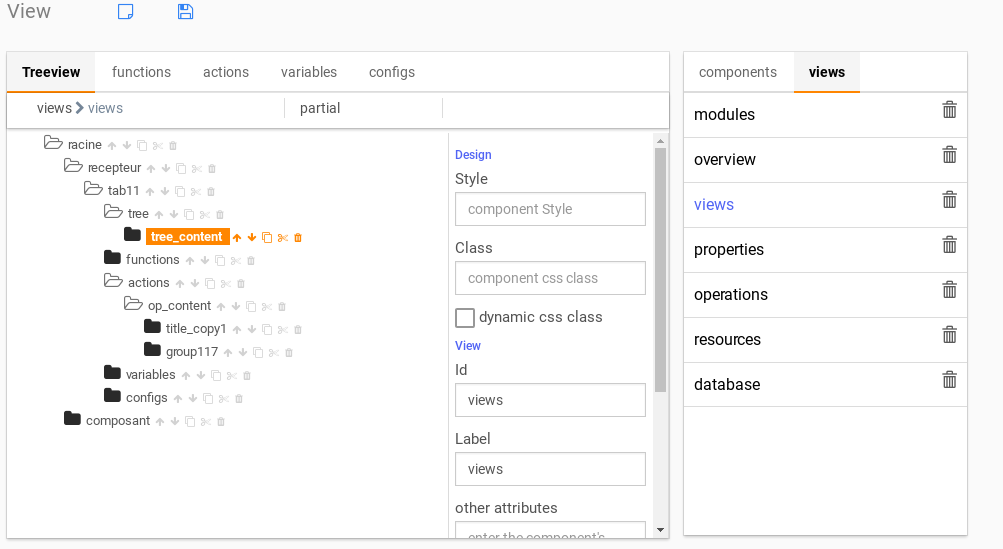
\includegraphics [width=0.90\textwidth] {./images/view.png}
 
  \item operations \\
 \\
 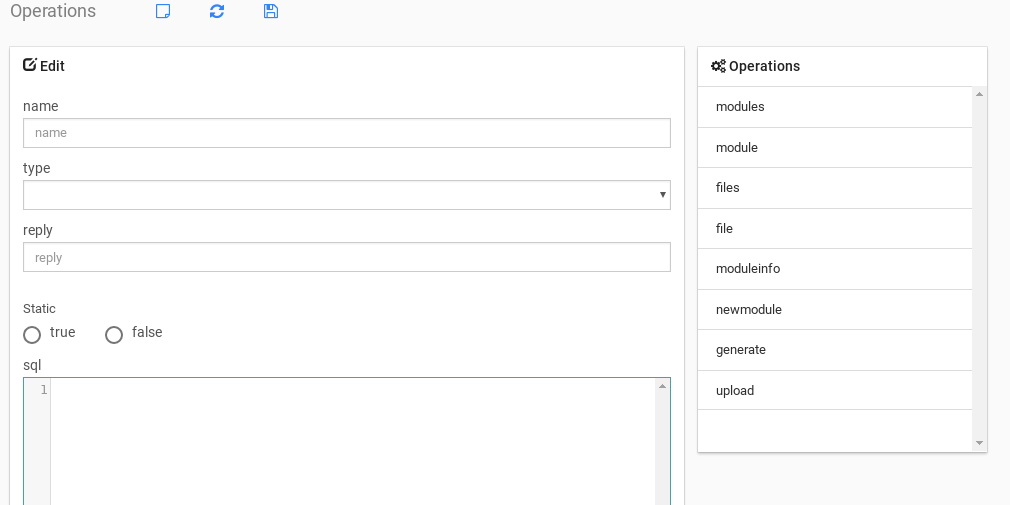
\includegraphics [width=0.90\textwidth] {./images/operations.png}
 
 \item resources \\
 \\
 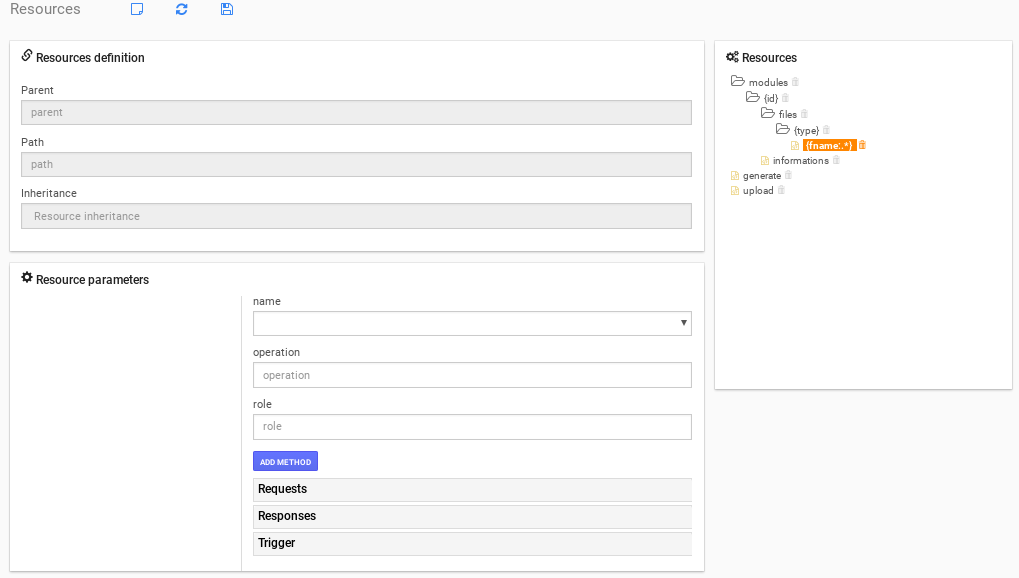
\includegraphics [width=0.90\textwidth] {./images/resources.png}
 
\end{itemize}



\subsubsection{Le générateur de vues}

\subsection{Les ressources}
%% présenter les différentes ressources et leurs opérations associées


\subsection{La base de données}

\subsection{La collaboration}
%% parler de gitolite et de la manière dont on crée des branches pour
%% le module


\chapter{conclusion}


\end{document} 
